% Shared preamble for the English summaries in this repository.
\documentclass[11pt,a4paper]{article}
\usepackage[margin=2.2cm]{geometry}
\usepackage[T1]{fontenc}
\usepackage[utf8]{inputenc}
\usepackage{lmodern}
\usepackage{amsmath,amssymb}
\usepackage{graphicx}
\usepackage{booktabs}
\usepackage{enumitem}
\usepackage[hidelinks]{hyperref}
\setlist{itemsep=2pt,topsep=4pt}
\setlength{\parindent}{0pt}
\setlength{\parskip}{5pt}
\graphicspath{{figures/}}
\newcommand{\summaryheader}[3]{%
  \begin{center}
    {\Large\bfseries #2}\\[3pt]
    {\large #1}\\[3pt]
    {\small Arshia Goshtasbi \textbullet{} MSc Electrical Engineering (Control), Iran University of Science and Technology \textbullet{} #3}
  \end{center}
  \vspace{2pt}\hrule\vspace{8pt}
  \noindent\textit{English summary of my original Persian report, which is kept as a PDF in this folder.}\par}

\begin{document}
\summaryheader{Optimal Control, Homework 6}{Minimum-time Bang-bang Control versus State Feedback (Kirk Example 5.4-4)}{Spring 1404 (2025)}

\section*{(a) Minimum-time control (\texttt{Q5\_4\_4\_A.slx})}
For the second-order plant with $|u|\le 1$, Pontryagin's principle gives a bang-bang control that switches on a switching curve. I put the switching law in a MATLAB Function block and simulated four initial states. The times to reach the origin, read from my report and the plots:
\begin{center}
\begin{tabular}{lcccc}\toprule
Initial state $(x_1,x_2)$ & $(-2,2)$ & $(2,-2)$ & $(4,-2)$ & $(-4,-2)$\\\midrule
Minimum time (s) & 2 & 2 & 2.9 & 6.9\\\bottomrule
\end{tabular}
\end{center}
\begin{center}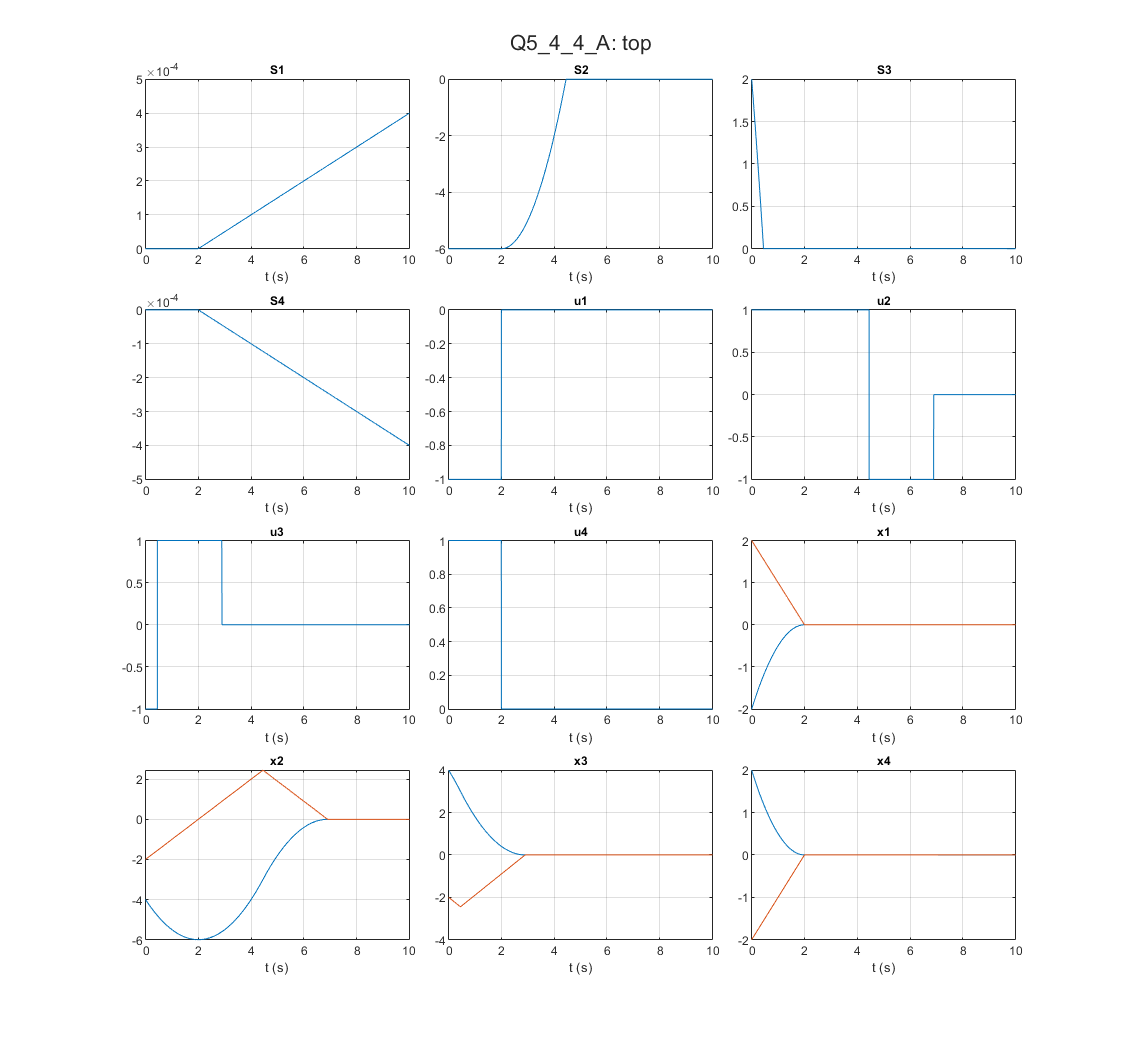
\includegraphics[width=0.75\linewidth]{Q5_4_4_A_scopes.png}\end{center}

\section*{(b) Linear state feedback with poles at $-1\pm j$ (\texttt{Q5\_4\_4\_B.slx})}
I designed a state feedback that places the closed-loop poles at $-1\pm j$ and simulated the same four initial states. The response is smooth, but it reaches the origin in about 8\,s for the first two states and about 9\,s for the third. The fourth did not reach the origin within the 10\,s simulation.
\begin{center}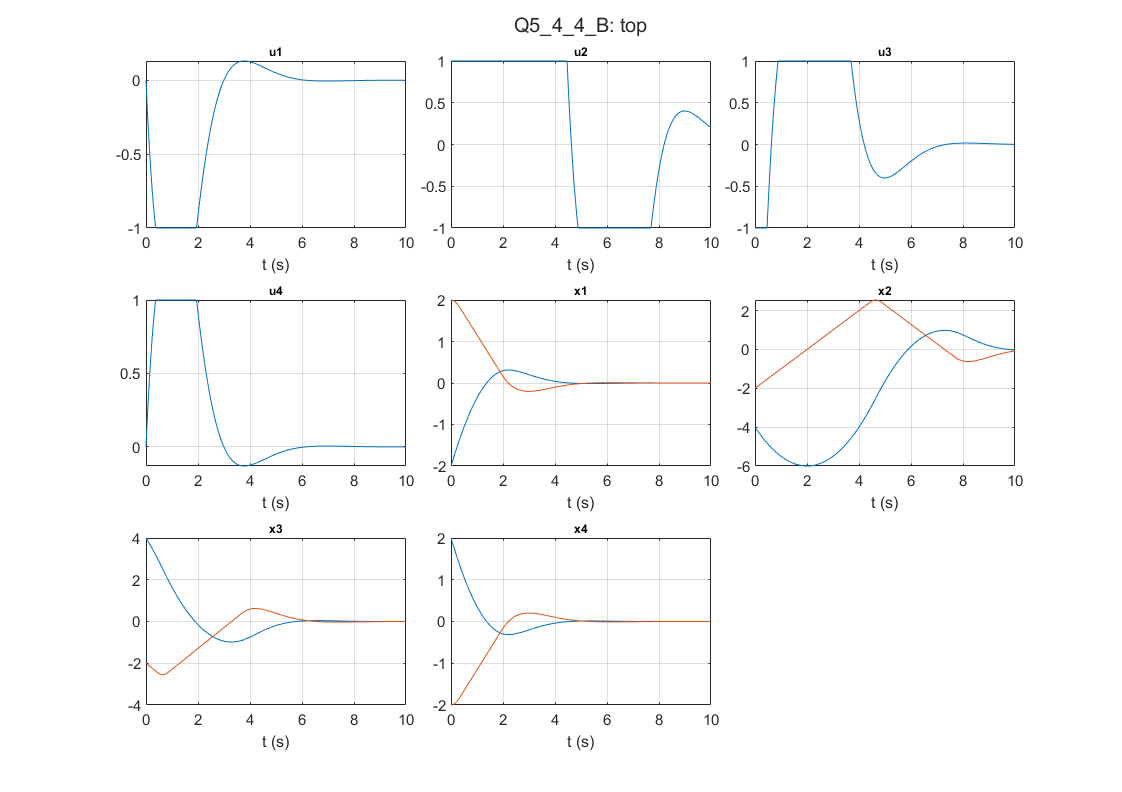
\includegraphics[width=0.62\linewidth]{Q5_4_4_B_scopes.png}\end{center}

\section*{Conclusion}
Under the same input bound, the bang-bang law from Pontryagin's principle reaches the origin much faster, because it always uses the full control authority. The linear state feedback is simpler, but it is clearly slower for every initial state.
\end{document}
